\chapter{Implementation, Testing and Deployment}
\label{impltesting}

\label{sec:impl}
\section{Introduction}

This chapters deals with the implementation of the application, with the focus on the application entities, and how they were configured.

\section{Application Entities}
\subsection{Users - Persistence}

The \textit{User} class represents every user account within the application. This section will focus on a regular user, how it is configured within the application in terms of bean definition and persistence. 

Firstly, as shown in line one of Figure ~\ref{fig:userDef}, the class needs to be configured as a \textit{Component} for the application. This ensures that the Spring framework considers the User class as one for auto-detection, through the use of class path scanning and annotations prevalent within this application. The framework instantiates this bean, or object, automatically, without the developer having to use the \textit{new} keyword.

\begin{figure}[H]
\begin{lstlisting}
@Component
@Entity
@Table(name="users")
public class User {
	@Id
	@GeneratedValue
	int id;
	
	@NotNull(groups={PersistenceValidationGroup.class, FormValidationGroup.class})
	@Pattern(regexp=".+\\@.+\\..+", message="This does not appear to be a valid email address", groups={PersistenceValidationGroup.class, FormValidationGroup.class})
	@Column(name="username")
	String username;
	
	@Size(min=5, max=45, message="Named must be between 5 and 45 characters",groups={PersistenceValidationGroup.class, FormValidationGroup.class})
	@Column(name="name")
	String name;
	
	@Column(name="password")
	@Size(min=5, max=15, message="Password must be between 5 and 15 characters", groups=FormValidationGroup.class)
	String password;
	
	@Column(name="gender")
	String gender;
	
	@Pattern(regexp="08[35679]([0-9]{7})", message="Number must be in the format 083, 085, 086, 087, 089 and 7 additional numbers eg 0851234567", groups={PersistenceValidationGroup.class, FormValidationGroup.class})
	@Column(name="contact_num")
	String contact_num;
	//Class truncated. Some repetitive attributes omitted
	//Getters and Setters below here.
\end{lstlisting}
\caption{User Class Definition and Configuration}
\label{fig:userDef}
\end{figure}

The \textit{Entity} and \textit{Table} annotations of lines 2 and 3 respectively belong to the javax.persistance package. These annotations are used by Hibernate in order to manage and persist the class. The \textit{@Table} annotation has a 'name' attribute that refers to the schema table the class maps to. There are two ways that an attribute can be assigned to a table column by Hibernate. Both methods are shown in Figure ~\ref{fig:userDef}. An annotation may be placed on the attribute in order to specify a column name. Line 11 in Figure ~\ref{fig:userDef} shows the username attribute being mapped to the username column within the User database schema. The other way of specifying where an attribute should be persisted is to ensure that the attribute name matches the column name within the table. This implicitly allows Hibernate to map a class, without having to explicitly define the mapping for the persistence framework.

The User class has a number of attribute constraints placed upon it. There are two types of constraints within this application: \textit{FormValidationGroup} and \textit{PersistenceValidationGroup}. These are interface classes with no attributes that serve as identifiers. As shown in lines 10, 14, 19 and 25 of Figure ~\ref{fig:userDef}, an attribute may be constrained by one or more groups. An annotation, from the javax.validation.constraints, is applied to the attribute. The annotations used within this application are as detailed in Table ~\ref{fig:classConstraints}.

\begin{table}[H]
\caption{Class Constraints}
\begin{center}
    \begin{tabular}{ | l | l | p{5cm} |}
    \hline
    Constraint Name & Description\\ \hline
	NotNull [Line 9] & Ensures the value within the attribute does not have a null value\\ \hline
	Pattern [Line 10] & Ensures the value within the attribute conforms to a regular expression\\ \hline
    @Size - Min [Line 14] & Ensures the value within the attribute has a minimum length\\ \hline
	@Size - Max [Line 14] & Ensures the value within the attribute has a maximum length\\ \hline

    \end{tabular}
\end{center}

\label{fig:classConstraints}
\end{table}

These validation package interfaces provide a \textit{groups} attribute, which is an array of objects. The \textit{FormValidationGroup} and \textit{PersistenceValidationGroup} are passed to this attribute. These groups allow attributes to have different constraints at different stages in the application. When using this attribute within the application, such as the creation of a user within a form, the Controller classes apply the validation to the user input and persisted data. The reason for having two groups of validation within this application is due to security. In every application, it is advisable to perform encryption on sensitive data, such as passwords. Within the scope of this application, user passwords were defined as being between 5 and 15 characters long, with no restriction to the content of the password. This application flow on taking in user input and persisting it is demonstrated below in Figure~\ref{fig:dbflow}.

\begin{figure}[H]
\begin{center}
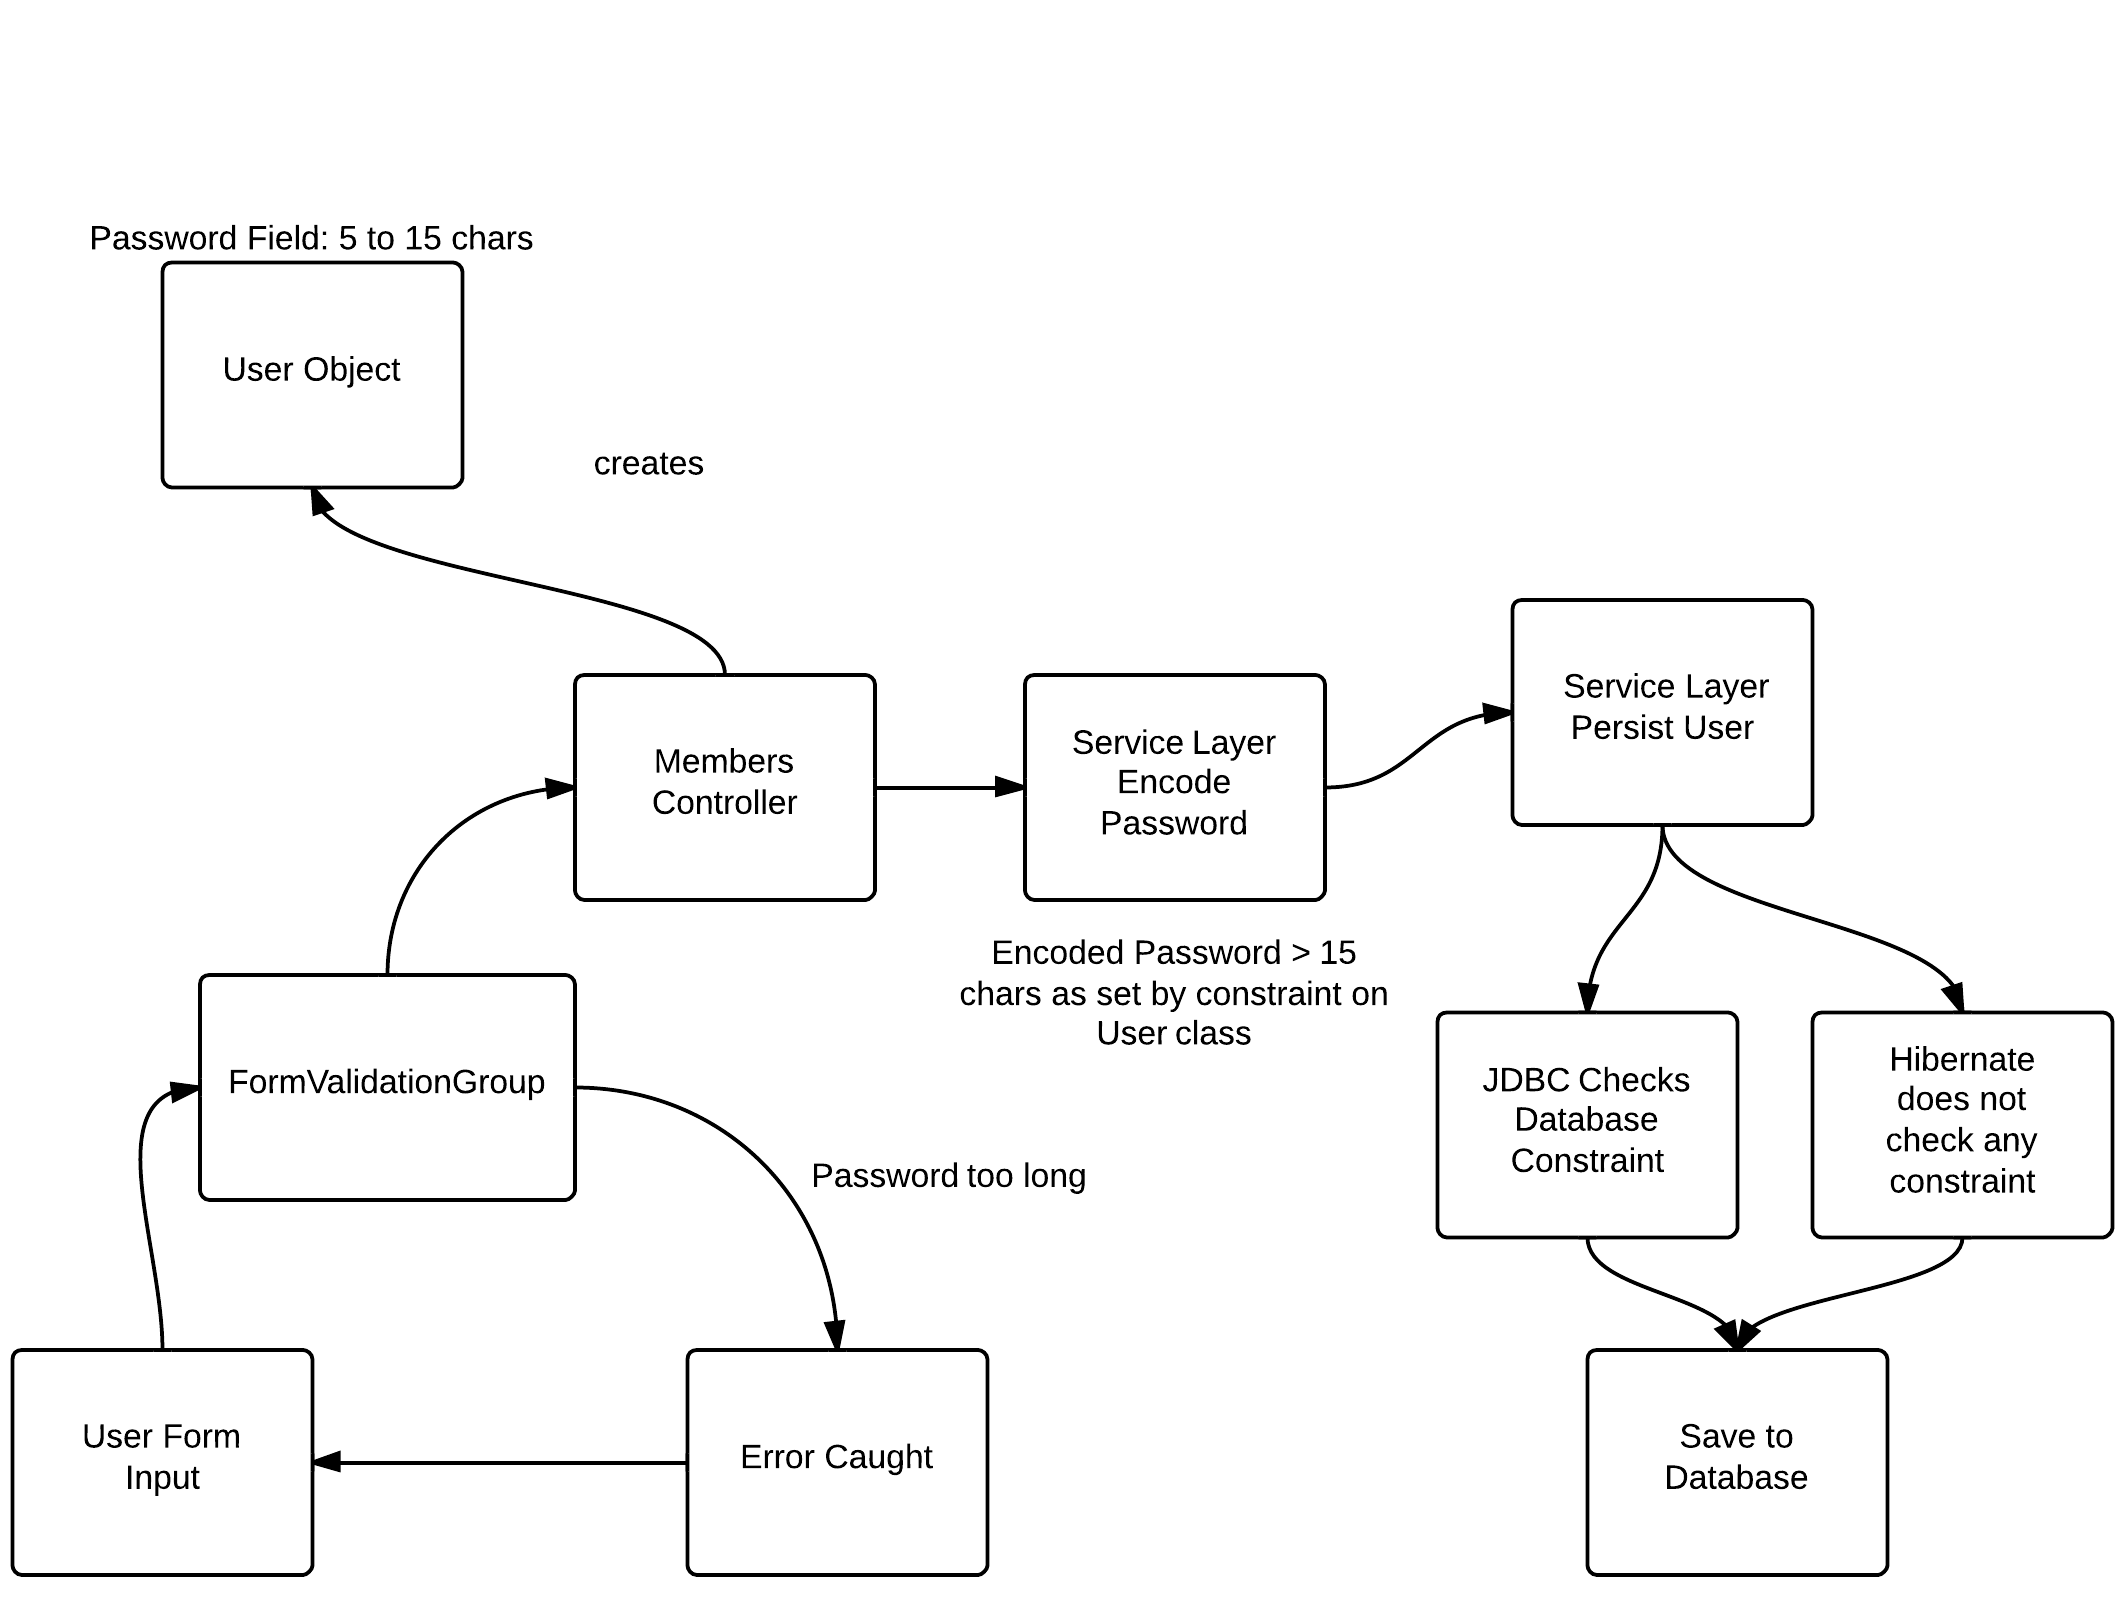
\includegraphics[width=14cm]{dbflow.png}
\end{center}
\caption{Application flow to persist User object}
\label{fig:dbflow}
\end{figure}

For example, a user password with 8 characters would pass form validation with no issues. When the PasswordEncoder bean is applied to the string prior to persistence, it will result in a value like \textit{'acb172137243c0b931321d7645dc31c2efb8346385ae0547d11b1d8de333215b'}, a value much longer than 15 characters. This will cause a failure with Hibernate persistence. This is because Hibernate works at a class level, and does take note of the constraints placed upon the class, while JDBC does not. The constraints that JDBC takes note of are those taken directly from the database itself. In this application, passing form validation is sufficient, as there are security annotations placed on the Service classes that manage data persistence. An example of how the controller handles validation is shown later in Figure ~\ref{fig:memberController}. 

Alongside class configuration, it is also necessary to configure Hibernate to scan the packages that contain entities, as detailed in Figure ~\ref{fig:hibernateConfig}. This is done through the creation of a sessionFactory bean, which uses the AnnotationSessionFactoryBean class. This bean is responsible for the creation of session instances within the application, though each application usually only has one session. It is an immutable object, and cannot be changed once it is created, so proper configuration of classes to facilitate object-relational mapping is important. The Session object created by the factory is responsible for creating the connection between the application and the database.

\begin{figure}[H]
\begin{lstlisting}
<bean id="sessionFactory"
class="org.springframework.orm.hibernate3.annotation.AnnotationSessionFactoryBean">
<property name="dataSource" ref="dataSource"></property>
<property name="hibernateProperties">
	<props>
		<prop key="hibernate.dialect">org.hibernate.dialect.MySQL5Dialect</prop>
	</props>
</property>
<property name="packagesToScan">
	<list>
		<value>users</value> 
		<!-- user refers to a package that contains user related classes --!>
	</list>
</property>
</bean>
\end{lstlisting}
\caption{Hibernate SessionFactory Configuration}
\label{fig:hibernateConfig}
\end{figure}

The HibernateProperties property defined in Line 4 refers to the SQL dialect used by Hibernate. This dialect provides the functionality to use human readable expressions to define query statements. Hibernate does not use SQL to structure these statement. It uses a variant called Hibernate Query Language [HQL]. HQL syntax is based has its basis in object oriented programming. The class itself defines the table, not the syntax. The difference in implementation is shown in Figure~\ref{fig:hqlsql}.

\begin{lstlisting}
SQL [JDBC]: jdbc.query("select * from users", new UserRowMapper());
// UserRowMapper is a class that maps rows to objects
HQL [Hibernate]: session().createQuery("from User").list;
\end{lstlisting}
\begin{figure}[H]
\caption{HQL-SQL Comparison}
\label{fig:hqlsql}
\end{figure}
 
The Form Validation is provided by the Spring Security file, which will be examined in detail in the Administration Implementation section on page ~\pageref{sec:adminImp}. As discussed previously, there are a number of validation constraints placed on the \textit{User} class. Spring provides a facility to ensure these constraints are enforced, and to also provide a positive user experience. It does this through the use of a BindingResult object. This object holds a record of any errors from the form that the user populates. The controller that deals with the form will check the BindingResult object for errors, and can respond appropriately. In order for this to work, both the Controller and the form, as depicted in Figures~\ref{fig:memberForm} and~\ref{fig:memberController}, need to be defined clearly. The form needs to be created  using the Spring Framework form tag library, and errors needs to be specified for each input within the form. 

\begin{figure}[H]
\begin{lstlisting}
<!-- Excerpt from the User registration form. Formatting removed for clarity --!>
<sf:form id="details" method="post" action="${pageContext.request.contextPath}/register" commandName="member">
Name <sf:input name = "name" path="name" type="text"/>
<sf:errors path="name" cssClass="error"></sf:errors>
Password <sf:input id="password" name = "password" path="password" type="password"/>
<sf:errors path="password" cssClass="error"></sf:errors>
</sf:form>
\end{lstlisting}
\caption{User Registration Form}
\label{fig:memberForm}
\end{figure}

The form structure, illustrated partially in Figure~\ref{fig:memberForm}, contains a number of important attributes. The form used is an extended version of the HTML <form> object. The Spring MVC version adds extra functionality such as mapping to objects within the controller classes and error validation checking. The \textit{commandName} is a variable within the form that contains the information within the form. This temporarily persists data between the form and the controller. This benefits the user as the application repopulates valid fields in the form should an error be made. The \textit{sf:error} tags allow the controller to identify specific errors within the form. These also reference attributes within the class the form is linked with. In this example, the \textit{User} class is being created with this form. 

Figure~\ref{memberController} Line 4 shows the declaration of a BindingResult object. This object holds the results of the form validation. Line 5 declares that if the result object has any errors, the controller returns to the form, where the \textit{sf:error} tags will highlight the error message relation to any attributes that broke their constraints. Lines 9 through 13 show home the application ensures that the primary key remains unique. 

\begin{figure}[H]
\begin{lstlisting}
//Method from the MembersController class
//This method is responsible for validating the form that users complete to register.
@RequestMapping(value = "/register", method = RequestMethod.POST)
public String doRegister(Model model,
@Validated(FormValidationGroup.class) @ModelAttribute("member") User member, BindingResult result) {
if (result.hasErrors()) {
	return "createmembers"; // if the result has errors, go back to create page
}
if (userService.exists(member.getUsername())) {
	result.rejectValue("username", "Duplicate Key",
	"This email address has already been used");
	return "createmembers";
	//if the email address already exists, return with this message.
}
	else {
		try {
			member.setAuthority("ROLE_MEMBER");
			userService.create(member);
			return "registerSuccess";
			//successful creation of member
			} catch (Exception e) {
				return "error";
			}
		}
}
\end{lstlisting}
\caption{User Registration Controller}
\label{fig:memberController}
\end{figure}

Line 13 in Figure~\ref{fig:memberController} shows the use of a \textit{ModelAttribute}. A \textit{ModelAttriute} is a property of the model that is supplied by Spring MVC to the controller. This object is created using the data mapped from the preceding form. This object is being validated using the \textit{FormValidationGroup} as specified using the \textit{Validated} annotation.

Within this application, the Service layer is responsible for the Controller communicating with the DAO layer to persist objects like the User class. Since Hibernate is configured at a class level, in relation to attributes and column names, there is no need for any INSERT or UPDATE statements. The current session, see Figure ~\ref{fig:getSession} is returned to the DAO object via the configured bean, and the necessary methods, such as save() and delete(), are called upon it. An object must be passed to the \textit{save()} method of the current sessionFactory object, detailed in ~\ref{fig:hibernateConfig}. 

\begin{figure}[H]
\begin{lstlisting}
public Session session(){
	logger.info("Session Factory returning current session.....");
	return sessionFactory.getCurrentSession();
}
\end{lstlisting}
\caption{UserDAO getSession()}
\label{fig:getSession}
\end{figure}

In the case of the User object, the password needs to be encoded prior to the object being persisted by the session(). In order to encode password, a bean responsible for the encoding must be defined within the application context, illustrated in Figure ~\ref{fig:passwordEncoder}. Spring provides a class that allows passwords to be encoded, and the bean for this class is defined within a security-context file.

\begin{figure}[H]
\begin{lstlisting}
<bean id="passwordEncoder"
class="org.springframework.security.crypto.password.StandardPasswordEncoder">
</bean>
\end{lstlisting}
\caption{Password Encoder Definition}
\label{fig:passwordEncoder}
\end{figure}

This Spring defined class provides an implementation for encoding data using SHA-256 hashing with 1024 iterations, with a random 8 byte salt value. This object then calls \textit{encode()} on the value passed from the form filled by the user. As a result, the actual password is never stored in the database, just an encrypted form of it, as shown in Figure ~\ref{fig:userPersist}. Once the password is encoded (Line 4, ~\ref{fig:userPersist}), the session() object can save the object. Due to the class configuration, there is no need to specify any database schema information within the DAO classes.

\begin{figure}[H]
\begin{lstlisting}
@Transactional
public void createUser(User user) {
	user.setPassword(passwordEncoder.encode(user.getPassword()));
	session().save(user);
}
\end{lstlisting}
\caption{Persisting User object with encoded password}
\label{fig:userPersist}
\end{figure}

\subsection{Timetable - Persistence Changes}

One of the most difficult features to implement within the application was the Timetable. While the goal was to create a timetable suitable for Monaleen Tennis Club, it was desirable that the timetable retain the portability and not rely on hard coded attributes. One issue arising from this constraint was the management of a varying varying number of slots in each day.A slot, within the scope of this application, is a portion of time in a day in which a booking can be made. If a user could define 10 slots a day, how would be store this in such a way that a user could also define a timetable with 20 slots a day? Hibernate was able to facilitate this design with considerably less input from a developer.

The solution implemented in this application was to use List objects to store the values for each day. There would be seven lists in the Timetable class, one for each day, as per Figure ~\ref{fig:timetableConfig}.


\begin{lstlisting}
@Entity
@Component
@Table(name = "timetable")
public class MonaleenTTV1 implements Timetable {
	@Id
	@GeneratedValue
	private int id;
	/**
	* Other Attributes Here
	**/
	
	@ElementCollection
	@CollectionTable (name = "monday", joinColumns=@JoinColumn(name="id"))
	private List<String> monday;
	
	@ElementCollection
	@CollectionTable (name = "tuesday", joinColumns=@JoinColumn(name="id"))
	private List<String> tuesday;
	
	@ElementCollection
	@CollectionTable (name = "wednesday", joinColumns=@JoinColumn(name="id"))
	private List<String> wednesday;
	
	@ElementCollection
	@CollectionTable (name = "thursday", joinColumns=@JoinColumn(name="id"))
	private List<String> thursday;
	
	@ElementCollection
	@CollectionTable (name = "friday", joinColumns=@JoinColumn(name="id"))
	private List<String> friday;
	
	@ElementCollection
	@CollectionTable (name = "saturday", joinColumns=@JoinColumn(name="id"))
	private List<String> saturday;
	
	@ElementCollection
	@CollectionTable (name = "sunday", joinColumns=@JoinColumn(name="id"))
	private List<String> sunday;
	
	//getters and setters
}
\end{lstlisting}
\begin{figure}[H]
\caption{Timetable Class List Configuration}
\label{fig:timetableConfig}
\end{figure}

This results in the Timetable object being made up of 8 database tables. The core of the class is stored in the 'Timetable' database table. This table contains the primary keys and all other attributes, such as name, number of slots, timetable series. The seven other tables each represent a collection within the Timetable class. Each of these tables has a non unique, foreign key that ties it back to the central table. This is illustrated in Figure~\ref{fig:timetableConfig} with use of the \textit{CollectionTable} annotation. This annotation defines the table that each collection belongs to. It also specifies a column for the HQL and SQL JOIN statement in the \textit{JoinColumn} annotation. For example, if we were to create a Timetable with 10 slots, with the primary key being 1, each of the collection tables would have 10 entries. Each of these entries would have an id of 1, to match the primary key in the core table, plus a value, such as 'Free Court'. The position in the table corresponds to the position within the collection class. 

The example, in Figure ~\ref{fig:ttdb}, shows a timetable configured with two slots. Upon creation, a series is created for each timetable. Each series contains 52 timetables, one for each week. The currently displayed timetable is determined by its position in the series in relation to the current week of the year, as shown by the Java Calendar class. The 'preview' attribute determines how far ahead the application will allow the user to browse in a timetable series. By default, the application displays the current weeks timetable, and does not allow a user to go backwards. If the current week, as defined by the Java Calendar class, is 13, the user will be able to see weeks 14, 15 and 16, owing to the preview with a value of 3. In Table~\ref{fig:ttdb}, the next three weeks of timetables are available for viewing and booking. This allows the administrator to dynamically restrict how far in advance users can book slots.

\begin{table}[H]
	\caption{Timetable Core Database Table}
    \begin{tabular}{| l | l | l | l | l | l | l | l | p{.8cm} |}
    \hline
    pid & name & slots & startTime & endTime & enabled & preview & series & total\\ \hline
    1 & Court One Week 1 & 2 & 8 & 22 & 1 & 3 & 1 & 52\\ \hline
	2 & Court One Week 2 & 2 & 8 & 22 & 0 & 3 & 1 & 52\\ \hline
	3 & Court One Week 3 & 2 & 8 & 22 & 0 & 3 & 1 & 52\\ \hline
	4 & Court One Week 4 & 2 & 8 & 22 & 0 & 3 & 1 & 52\\ \hline
    \end{tabular}

	\label{fig:ttdb}
\end{table}

\begin{table}[H]f
	\caption{Timetable Storage Table for Monday Collection}
\begin {center}
    \begin{tabular}{| l | l | p{.8cm} |}
	\hline
	pid & monday \\ \hline
	1 & Free Court \\ \hline
	1 & Free Court \\ \hline
	2 & Tournament \\ \hline
	2 & Free Court \\ \hline
	3 & User Booking \\ \hline
	3 & Free Court \\ \hline
	4 & Training \\ \hline
	4 & Free Court \\ \hline
	\end{tabular}
	\end{center}
\end{table}

The above tables shows 4 timetables, and the events that occur on a Monday. Timetable 1 has the events 'Free Court' and 'Free Court', while Timetable 4 has 'Training' and 'Free Court'. The amount of entries in determined by the number of slots specified when the timetable is created. 

While the table structure of the \textit{User} and \textit{Timetable} differ considerably, since Hibernate deals with objects, that have table structures defined within their classes, there is no change to the way the Timetable is saved and updated, as per Figure ~\ref{timetableHibernate}. Using JDBC, there would have been 8 SQL queries to save to each of the 8 table, increasing the risk of bugs within the application, or invalid data being saved or retrieved.

\begin{figure}[H]
\begin{lstlisting}
@Transactional
public void createTimetable(Timetable t) {
	session().save(t);
}
\end{lstlisting}
\caption{Hibernate Save Timetable}
\label{fig:timetableHibernate}
\end{figure}

The timetable is displayed in the application as shown in Figure~\ref{fig:timetablesite}.

\begin{figure}[H]
\begin{center}
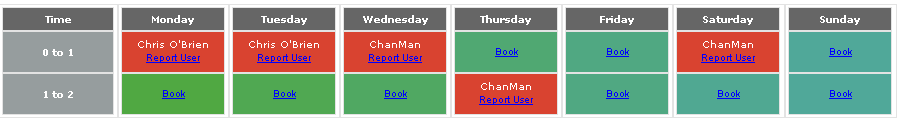
\includegraphics[width=15cm]{timetable.png}
\end{center}
\caption{Timetable snapshot within the application}
\label{fig:timetablesite}
\end{figure}


\subsection{Tournaments and Timetable Events}

The third major area of the site were the \textit{Tournament} and \textit{Event} classes. The structure and configuration of these classes are not different from the \textit{User} or \textit{Timetable} classes. In the context of this report and application, an Event is any object that can populate a field within a Timetable class. 

\subsubsection{Events}

Within the scope of this application, an \textit{Event} is any item that can be scheduled within the Timetable object. As with the \textit{Tournament} class, the \textit{Event} class is configured much like the \textit{User} and \textit{Timetable} classes. One event that is required by all versions of the Timetable is the 'Free Court' event. This event is created by default (see Figure ~\ref{fig:createEvent}) either the first time an administrator attempts to create an Event, or to create a Timetable. An Event has two attributes: a name and an author. In the case of a system event, the name will be the login of the person who booked the timetable slot, while the author is defined as \textit{BOOKING SYSTEM}. For an administrator event, the name is defined by that administrator, while the author is listed as the administrator who created the event. Example events for Monaleen Tennis would be:

\begin{itemize}
\item Training Sessions
\item Club Social Events
\item Ladies Tennis
\item Recurring Tournaments
\item General Club Activities
\end{itemize}

\begin{lstlisting}
@RequestMapping(value = "/saveEvent", method = RequestMethod.POST)
public String saveEvent(Model model, @ModelAttribute("event") Event e,
	BindingResult result) {
	if (eventService.getEventById(1).equals(null)){
		e.setName("Free Court");
		e.setAuthor(userService.emailToName(SecurityContextHolder
		.getContext().getAuthentication().getName()));
		e.setEnabled(true);
		eventService.createEvent(e); // see Line 29-32 for creation of Event.
	}
	logger.info("Event Save Method....");
	if (result.hasErrors()) {
		return "createEvent";
	}
	if (eventService.exists(e.getName())) {
		result.rejectValue("name", "Duplicate Key",
		"This Event Name has already been used.");
		return "createEvent";
	} else {
		e.setAuthor(userService.emailToName(SecurityContextHolder
		.getContext().getAuthentication().getName()));
		e.setEnabled(false);
		eventService.createEvent(e);
		return viewEvent(model);
	}
}

//Event DAO 
public void createNewEvent(I_Event e){
	logger.info("Creating new event....");
	session().save(e);
}
\end{lstlisting}
\begin{figure}[H]
\caption{Event Creation}
\label{fig:createEvent}
\end{figure}

Lines 4 through 10 are necessary to ensure no NullPointerExceptions are introduced when creating a timetable. If no events exist within the system either the first time a timetable is created or, as illustrated above in Figure~\ref{fig:createEvent}, the system will create a \textit{Free Court} event which is needed for the timetable to function correctly.

In order for an event to show up as an option when creating, or editing, a timetable, it must be enabled, as shown in Figure ~\ref{fig:enableEvent}. This implementation allows the administrator to pre-create events for later use without overcrowding the timetable.

\begin{lstlisting}
@RequestMapping("/changeEventStatus")
public String changeEventStatus(Model model, HttpServletRequest request) {
	Event e = (Event) eventService.getEventById(Integer.valueOf(request
	.getParameter("eventID")));
	if (e.isEnabled()) {
		e.setEnabled(false);
		eventService.updateEvent(e);
		return viewEvent(model);
	} else {
		e.setEnabled(true);
		eventService.updateEvent(e);
		return viewEvent(model);
	}
}
\end{lstlisting}
\begin{figure}[H]
\caption{Change Event Status}
\label{fig:enableEvent}
\end{figure} 	

\subsubsection{Tournament}

The \textit{Tournament} class is configured similar to the \textit{Timetable} class, in that it has a secondary table which contains a list of members who have registered for the tournament. The key area for tournament implementation was for the application to differentiate between the various states of the tournament, such as registration being enabled, yet the tournament not having started yet. This process is shown in Figure~\ref{fig:tourstate} It was also important that the tournament could link up with the Timetable system, in order to book slots to play the tournament. In this regards, a tournament was required to manage an Event object, see Figure~\ref{fig:tourCreate}, and to ensure that no ambiguity was present when dealing with multiple tournaments and possible multiple timetables. It was also necessary for a Tournament object to manage its own event in order to minimise both the risk of ambiguity and administration involvement.


\begin{center}
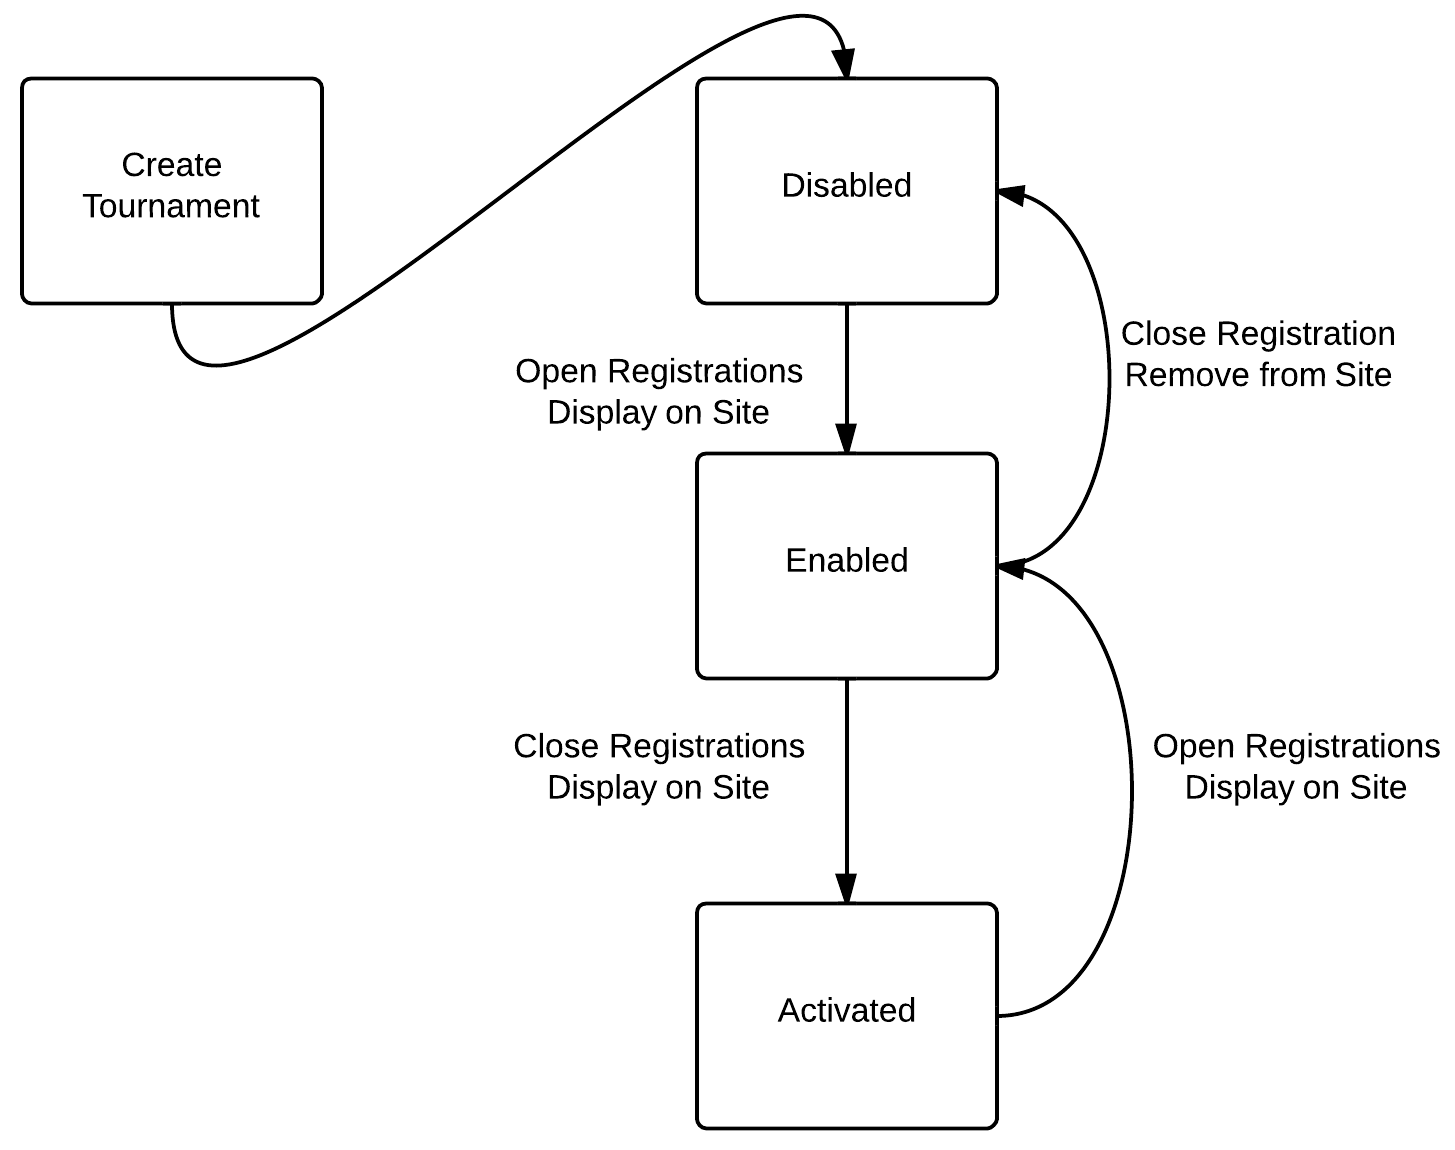
\includegraphics[scale=0.3]{tourstate.png}
\end{center}
\begin{figure}[H]
\caption{Tournament State Chart}
\label{fig:tourstate}
\end{figure}


\begin{lstlisting}
@RequestMapping(value = "/registerTournament", method = RequestMethod.POST)
public String doCreateTournament(
	Model model, BindingResult result,
	@Validated(FormValidationGroup.class) @ModelAttribute("tournament") Tournament t) {
	
	if (result.hasErrors()) {
		return "createTournament";
	} 
	if (tournamentService.exists(t.getTournamentName())){
		if (eventService.exists(t.getTournamentName())){
		result.rejectValue("tournamentName", "Duplicate Key",
		"An event of this name already exists");
		return "createTournament";
	}
	result.rejectValue("tournamentName", "Duplicate Key",
		"A tournament of this name already exists");
		return "createTournament";
		}
	else {
		try {
			tournamentService.create(t);
			eventCreation(t);
			logger.info("Tournament Created");
			return "tournamentSuccess";
		} catch (Exception e) {
		return "error";
	}
}
public void eventCreation(Tournament t){
	Event e = new Event();
	e.setName(t.getTournamentName());
	e.setAuthor(userService.emailToName(SecurityContextHolder.getContext()
	.getAuthentication().getName()));
	eventService.createEvent(e); 
	// this method invokes the createEvent() method within the service class
	// the service layer then called on the EventDAO object to persist the Event
}
\end{lstlisting}
\begin{figure}[H]
\caption{Tournament Creation}
\label{fig:tourCreate}
\end{figure}

Deleting a tournament needed similar logic, as displayed in Figure ~\ref{fig:deleteTour}. Similar to the \textit{User} class, the Tournament name, much like the username, is used as a primary key, and can be recycled once a tournament is deleted. 

\begin{lstlisting}
	@RequestMapping("/confirmDelete")
	public String deleteTournament(Model model, HttpServletRequest request){
		Tournament t = tournamentService.getTournamentById(request
				.getParameter("tournamentID"));
		tournamentService.deleteTournament(t);
		eventService.deleteEvent(eventService.getEventIdByName(t.getTournamentName()));
		model.addAttribute("tour", tournamentService.getAllTournaments());
		return "deleteTournament";
	}
\end{lstlisting}
\begin{figure}[H]
\caption{Delete Tournament}
\label{fig:deleteTour}
\end{figure}	

Due to constraints on time within the final year project, it wasn't possible to fully flesh out this area of the site, though it was implemented in such a way to allow for extensibility such as an interface for the sorting of registered members into teams. This interface would allow the specification of business logic to allow the system to, for example, sort tournament teams by experience and ranking. This interface, and the current implementation, in Figure~\ref{fig:tsort}.

\begin{lstlisting}
// Interface for Tournament Sorter
public interface I_TournamentSorter {
	public Map<String, String> sort(List<String> registered); //sorts tournament
	public boolean check(Tournament t); //checks if tournament can be sorted
}
//Implementation
public class BasicTournamentSort implements I_TournamentSorter {
//returns a Map of teams, odd number of persons results in one person
//getting no team
public Map<String, String> sort(List<String> registered) {
	Map<String, String> teams = new HashMap<String, String>();		
	if ((registered.size() % 2) != 0){
		teams.put("NoTeam", registered.get(registered.size()-1));
		registered.remove(registered.size()-1);
	}
	int j = 1;
	for (int i = 0; i < registered.size(); i++){
		teams.put("Team"+j, registered.get(i) + " & " + registered.get(i+1));
		i++;
		j++;
	}
		return teams;
}
//Checks to ensure at least two teams are registered
public boolean check(Tournament t) {
	if ((t.getUsername().size()) < 4){
		return false;
	}
	if (t.getTournamentType().equalsIgnoreCase("s")){
		return false;
	}
	else{
		return true;
	}
}
\end{lstlisting}
\begin{figure}
\caption{Existing Tournament Sort and Interface}
\label{fig:tsort}
\end{figure}

	
\label{sec:adminImp}
\subsection{Administration - Security and Session Management}

The \textit{Administration} section of the application deals with the implementation, and configuration, of the security and session management aspects of the application. An administrator has the same structure as a \textit{User} and is defined by the \textit{Role} it has, as seen previously in Figure ~\ref{fig:secRoles}. These roles are configured through Spring Security, in which a specific database schema must be adhered to. By default, there should be two tables: \textit{users} and \textit{authorities}, with a foreign key constraint. In this application, as shown in Line 3, Figure ~\ref{fig:roleConfig}, this was modified to keep the user data within the same table.

\begin{lstlisting}
<security:authentication-provider>
<security:jdbc-user-service data-source-ref="dataSource"
id="jdbcUserService" authorities-by-username-query="select username, authority from users where binary username = ?" />
<security:password-encoder ref="passwordEncoder"></security:password-encoder>
</security:authentication-provider>
\end{lstlisting}
\begin{figure}[H]
\caption{Spring Role Configuration}
\label{fig:roleConfig}
\end{figure}

The security within the application is controlled by the \textit{security-context.xml} file, which used Expression Based Access Control [EBAC] in order to restrict site access to relevant roles. EBAC allows complicated boolean logic to be encapsulated within a single expression, such as whether a user is authenticated or not. The base class used within this application is \textit{SecurityExpressionRoot}. These expressions are contained within the \textit{security-context.xml} file, as seen in Figure ~\ref{fig:secContext}. This configuration file is partly responsible for controller access to the mappings within the application. 

\begin{lstlisting}
<security:http use-expressions="true">
<security:intercept-url pattern="/static/**" access="permitAll" />
<security:intercept-url pattern="/images/**" access="permitAll" />
<security:intercept-url pattern="/createmembers" access="permitAll" />
<security:intercept-url pattern="/tournamentSuccess" access="hasAnyRole('ROLE_ADMIN', 'ROLE_COMMITTEE')" />
<security:intercept-url pattern="/createNews" access="hasAnyRole('ROLE_ADMIN', 'ROLE_COMMITTEE')" />
<security:intercept-url pattern="/members" access="isAuthenticated()" />
</security:http>
\end{lstlisting}
\begin{figure}[H]
\caption{Security Context File Excerpt}
\label{fig:secContext}
\end{figure}

An issue that arises with this implement ion is that all resources, such as images, would automatically be blocked from appearing on the site unless explicitly defined. In the case of images, this would be very time consuming, especially when new images are added to the application frequently. In order to overcome this, Lines 2 and 3 are implemented. This syntax specifies that all files and folders within the \textit{static} and \textit{images} folder are to be granted access to all pages within the application. Site access can also be granted on an authentication basis, rather than a role based system, and this is implemented as show in Line 7 of Figure~\ref{fig:secContext}.

In addition to the expression level security, service-level security annotations are also in place. This gives the application an extra layer of security, as it restricts the use of methods within the service layer to defined roles. It is possible to use either expression level security or service level security independently. This is configured within the \textit{security-context.xml} file, Figure ~\ref{fig:secAnnotate}, and is implemented, as shown in Figure ~\ref{fig:secAnonImpl}, within the service layer. These annotation use the same roles as defined previously within the application. 

\begin{lstlisting}
<security:global-method-security secured-annotations="enabled"></security:global-method-security>
\end{lstlisting}
\begin{figure}[H]
\caption{Security Context Service Layer Annotation Configuration}
\label{fig:secAnnotate}
\end{figure}

\begin{lstlisting}
@Service("timetableService")
public class TimetableService {

private TimetableDAO timetableDAO;

	@Autowired
	public void setTimetableDAO(TimetableDAO timetableDAO) {
		this.timetableDAO = timetableDAO;
	}
	
	@Secured("ROLE_ADMIN")
	public void create(Timetable t){
		timetableDAO.createTimetable(t);
	}
	
	@Secured({"ROLE_ADMIN", "ROLE_MEMBER", "ROLE_COMMITTEE", "ROLE_WARNING", "ROLE_SUSPEND"})
	public void update(Timetable t){
		timetableDAO.updateTimetable(t);
	}
	
	public List<Timetable> getAllTimetables(){
		return timetableDAO.listTimetables();
	}
}
\end{lstlisting}
\begin{figure}[H]
\caption{Security Context Service Layer Annotation Implementation}
\label{fig:secAnonImpl}
\end{figure}

In the implementation shown above, there are some items to note: the \textit{Service} and \textit{Autowired} annotations. The \textit{Service} annotation allows implementation classes to be auto-detected through class-path scanning. The package that contains the Service classes is defined within another XML file, \textit{service-context.xml} within this application, Figure ~\ref{fig:serviceContext}. This file configures Spring to look for Service classes via annotations, and where to look for them.

\begin{lstlisting}
<context:annotation-config></context:annotation-config>
<context:component-scan base-package="service"></context:component-scan>
\end{lstlisting}
\begin{figure}[H]
\caption{Service Context Configuration}
\label{fig:serviceContext}
\end{figure}

The \textit{Autowired} annotation is used within the framework to mark a constructor or setter. Spring then passes the needed dependencies into the application with its dependency injection facilities. 

\section{Model View Controller}
\subsection{Controller Layer}

A Controller is a class within the application that creates and modifies a model, and passes it onto a View. A View will also pass information to a Controller, which will communicate with the Service layer to persist any relevant data within the application.

A Controller is annotated, as illustrated in Figure~\ref{fig:controller}, Line 1. This allows the DispatcherServlet to identify the controllers and inject them into the application. This behaviour is displayed in Figure~\ref{fig:dscomponent}, which shows the DispatcherServlet being configured to scan the controllers package looking for annotations.

\begin{lstlisting}
@Controller
public class TimetableController {
	//.........
}
\end{lstlisting}
\begin{figure}[H]
\caption{Service Context Configuration}
\label{fig:controller}
\end{figure}

\begin{lstlisting}
<context:component-scan base-package="controllers, email"></context:component-scan>
<mvc:annotation-driven></mvc:annotation-driven>
\end{lstlisting}
\begin{figure}[H]
\caption{Service Context Configuration}
\label{fig:dscomponent}
\end{figure}

In order for the application to choose the correct method within a specific controller, it is necessary to define a mapping. The \textit{RequestMapping} annotation is used for this purpose. This annotation maps a web request onto a handler method within a controller, as depicted in Figure~\ref{fig:requestmapping}. It is also important, within the scope of the Spring Security configuration, to ensure that this mapping has access rights defined within the application or access will be denied.

\begin{lstlisting}
@RequestMapping("/")
public String showHome(Model model) {
	logger.info("Showing Home Page....");
	News news = newsService.getLatestStory();
	model.addAttribute("newsHeader", news.getSummary());
	model.addAttribute("newsContent", news.getContent());
	return "index";
}
\end{lstlisting}
\begin{figure}[H]
\caption{Request Mapping}
\label{fig:requestmapping}
\end{figure}

This mapping responds to a request with the value '/', Line 1. On Tomcat servers, the home page will be \textit{localhost:8080/application-name/}. In this example, the latest news story is retrieved on Line 4, and values from it are added to the model displayed on the returned view.

Any value specified after \textit{localhost:8080/application-name/} will search for a mapping within all controllers in the application. If a mapping does not exist, a resource not found will be displayed. This is default behaviour for a denied access attempt. In order to ensure the site can deal with invalid requests, an access denied handler can be defined within the Spring Security context file, as depicted in Figure~\ref{fig:accessDenied}. This allows a mapping to be specified for invalid requests.

\begin{lstlisting}
<security:access-denied-handler error-page="/denied" />
\end{lstlisting}
\begin{figure}[H]
\caption{Access denied Handler}
\label{fig:accessDenied}
\end{figure}

In this example, the \textit{denied} mapping, shown in Figure~\ref{fig:accessDenied} is called, and the corresponding view displayed, illustrated in Figure~\ref{fig:viewDenied}. 

\begin{lstlisting}
@RequestMapping("/denied")
public String showDeny(Model model){
	model.addAttribute("message", "The page you are looking for either does not exist, or you do not have access. Please contact an administrator if you believe this is an error.");
return "error";
}

//Error Page

<center>${message}</center>
\end{lstlisting}
\begin{figure}[H]
\caption{Error Page Mapping}
\label{fig:viewDenied}
\end{figure}

Line 3 shows a message being added to a model, which is added to a standard error page. This message will change depending on what error is being caught by the application. The message is then displayed by the 'error' View for the user, and the site appearance is not disrupted by a generic error page.

\subsection{Models within the Spring MVC Framework}

A model is a map containing a key-value pair that can be modified by a Controller and displayed by a View. A model is implicitly created by the framework by including a reference to it within the method signature in a controller, as illustrated in Figure~\ref{fig:modelDefine}. The example shown in Figure~\ref{fig:modelDefine} adds two lists to a model: a list of disabled events and a list of enabled events, shown in Lines 5 and 6. The Controller then returns the value \textit{viewEvents} to the ViewResolver. The ViewResolver displays the relevant page that displays the information held within the model for the user, as depicted in Figure~\ref{fig:modelJSP}

\begin{figure}[H]
\begin{lstlisting}
@RequestMapping("/viewEvents")
public String viewEvent(Model model) {
	List<Event> eventsDisabled = eventService.listDisabledEvents();
	List<Event> eventsEnabled = eventService.listEnabledEvents();
	model.addAttribute("eventsEnabled", eventsEnabled);
	model.addAttribute("eventsDisabled", eventsDisabled);
    return "viewEvents";
	}
\end{lstlisting}
\caption{Model Definition}
\label{fig:modelDefine}
\end{figure}

\begin{figure}[H]
\begin{lstlisting}
<c:if test="${not empty eventsEnabled }">
<table class="members" align="center">
<tr><th>Enabled Events</th></tr>
<tr>
<th>ID</th><th>Name</th><th>Author</th><th>Action</th></tr>
<c:forEach var="row" items="${eventsEnabled}">
<sf:form method="post"
action="${pageContext.request.contextPath}/changeEventStatus"
commandName="eventsEnabled">
<tr>
	<td><input type="hidden" value="${row.id}" name="eventID" />${row.id}</td>
	<td>${row.name}</td>
	<td>${row.author}</td>
	<td><input value="Disable" type="submit" name="${row.id}" />
</sf:form>
</c:forEach>
</table>
<center><font color="red">${message }</font></center>
</c:if>
\end{lstlisting}
\caption{JSP View of model}
\label{fig:modelJSP}
\end{figure}

The page contains a conditional loop, Line 1, that checks if the model attribute, eventsEnabled, is empty. If it is not, it will create a table to display the information to the user, as shown in Lines 2 through 17. The \textit{c:forEach} tag is the JSTL version of a for loop, which will be looked at in a later section. Line 18 is a message, that will display if the value is not null. This is used to display a confirmation or error message to the user when an action is performed on an event. An example would be an attempt to disable the \textit{Free Court} event. This will display a message, shown below in Figure~\ref{fig:modelFail}, that the action cannot be performed.

\begin{figure}[H]
\begin{lstlisting}
if (e.getName().equalsIgnoreCase("Free Court")){
	model.addAttribute("message", "You cannot modify the Free Court event");
	return viewEvent(model);
}
\end{lstlisting}
\caption{User message added to model}
\label{fig:modelFail}
\end{figure}

\subsection{View Layer}
\subsubsection{Apache Tiles Configuration and Implementation}
Apache Tiles is configured within the web application core XML file. There are two classes that the configuration is concerned with: TilesViewResolver and TileConfigurer. Both are declared as beans within the configuration file and automatically created when the application is launched. The primary function of the ViewResolver is to take in a String value, and return the relevant \textit{RequestMapping} value within the application. These mappings are defined within the Controller classes of the application. The TilesConfigurer object, see Figure ~\ref{fig:tilesXML}, takes one parameter: a location of the template that the default tile will use. The default tile will then be used by other pages as a template. \newline

\begin{figure}[H]
\begin{lstlisting}
<bean id="tilesViewResolver"
	class="org.springframework.web.servlet.view.tiles2.TilesViewResolver">
</bean>

<bean id="tilesConfig"
	class="org.springframework.web.servlet.view.tiles2.TilesConfigurer">
	<property name="definitions">
	<list>
		<value>/WEB-INF/layout/default.xml</value>
	</list>
	</property>
</bean>
\end{lstlisting}
\caption{Apache Tiles Configuration}
\label{fig:tilesXML}
\end{figure}

The default tile consists of a number of sections identified by a specific tag. These tags correspond to values within the tile layout configuration file. Using a version of inheritance, these can be overwritten and replaced with other pages in order to change the content of a page, while maintaining cohesion across the design of the application. 

The following examples shows the implementation within the configuration file. The first section of code is the overall template. This specifies the default values that make up a JSP page within the application. The second segment of code is the the definition for the initial home page for the web application. By the inclusion of the \textit{extends="users.base"} within the definition tags, it is defining the index as a sub class of the users.base definition. Consequently, it is possible to override any of the attributes within the users.base definition. In this example, the title and content of the default page are being overridden with different values in order construct a more suitable page. The header, links and footer however remain the same, and will do so will all pages following this format, as shown in Figure ~\ref{fig:tilesConfig}.

\begin{figure}[H]
\begin{lstlisting}
<definition name="users.base" template="/WEB-INF/templates/default.jsp">
	<put-attribute name="title" value="Monaleen Tennis Club - Default Template"></put-attribute>
	<put-attribute name="header" value="/WEB-INF/tiles/header.jsp"></put-attribute>
	<put-attribute name="links" value="/WEB-INF/tiles/links.jsp"></put-attribute>
	<put-attribute name="content" value="/WEB-INF/tiles/content.jsp"></put-attribute>
	<put-attribute name="footer" value="/WEB-INF/tiles/footer.jsp"></put-attribute>
</definition>

<definition name="index" extends="users.base">
	<put-attribute name="title" value="Monaleen Tennis Club - Home Page"></put-attribute>
	<put-attribute name="content" value="/WEB-INF/tiles/index.jsp"></put-attribute>
</definition>

<definition name="admin" extends="users.base">
	<put-attribute name="title" value="Monaleen Tennis Club - Admin"></put-attribute>
	<put-attribute name="content" value="/WEB-INF/tiles/admin.jsp"></put-attribute>
</definition>
\end{lstlisting}
\caption{Apache Tiles Configuration}
\label{fig:tilesConfig}
\end{figure}

\subsubsection{JSTL}

JSTL is used within the application to manage how information was displayed. It was preferred that all of the logic be handled at the Controller level, and that the JSP pages would resolve the models passed to it into the view seen by the user. It was not desirable for the pages to contain JSP directives, or to use the implicit objects contained within JSP pages. 

The main tags used within the application were the JSTL Core tags.  These tags allow the usage of conditional statements and the definition of parameters within the JSP page. In order to use this technology, the relevant jar must be made available in the build path or within the Maven dependencies of the project. A declaration, as shown in Figure ~\ref{fig:jstldec} must be included in all JSP pages that wish to make use of the tags also.\newline

\begin{figure}[H]
\begin{lstlisting}
<%@ taglib prefix="c" uri="http://java.sun.com/jsp/jstl/core"%>
\end{lstlisting}
\caption{JSTL Tag Library Declaration}
\label{fig:jstldec}
\end{figure}

Within the application, the controller will create a model and pass it to the JSP page. The page uses the JSTL tags to manage and display relevant information from the model, as shown in Figure ~\ref{fig:ttmodelattributes}, and user actions based on the information contained within. The example below is taken from the Timetable display page, Figure ~\ref{fig:ttcontrollerchoosecourt} from the application.\newline

\begin{lstlisting}
@RequestMapping(value = "/gotoCourt", method = RequestMethod.POST)
public String chooseCourt(Model model, HttpServletRequest request) {
	//abbreviated method to display court, logic removed
	//highlighting the attributes within the model
	model = addDateToTimetable(model, id));
	model.addAttribute("series",timetableService.getById(id).getSeries());
	model.addAttribute("name", SecurityContextHolder.getContext().getAuthentication().getName());
	model.addAttribute("court", current);
	model.addAttribute("realname", name);
	model.addAttribute("bookings", left);
	if (seriesMatch(courtID, nextCourt)) {
		model.addAttribute("next", (current.getId() + 1));
	}
	if (seriesMatch(courtID, prevCourt)) {
		model.addAttribute("prev", (current.getId() - 1));
	}
	return "court";
}
\end{lstlisting}	
\begin{figure}[H]
\caption{Timetable Controller chooseCourt() method}
\label{fig:ttcontrollerchoosecourt}
\end{figure}

\begin{table}[H]
\begin{center}
\caption{Model Attributes}
    \begin{tabular}{ | l | l | p{5cm} |}
    \hline
    Model Name & Summary \\ \hline
    name & The username of the currently authenticated user  \\ \hline
    realName & The real name of the currently authenticated user\\ \hline
	bookings & The number of remaining bookings of the currently authenticated users\\ \hline
	date & The current week of the year and the current date. Calculated using separate method.\\ \hline
	next & The id number of the court following the current court, if applicable\\ \hline
    prev & The id number of the court preceding the current court, if applicable\\ \hline
	court & The current court, determined by the current week, provided by the java.util.Date class \\
    \hline
    \end{tabular}
\end{center}

\label{fig:ttmodelattributes}
\end{table}

This example is an excerpt from the TimetableContoller class. The logic determining the values has been removed. This is to highlight how attributes are added to the model from within the controller. This is the information that the JSP page will have access to once it has been displayed.

The code in Figure~\ref{fig:ttmodelattributes} deals with the display of \textit{Monday} within the Timetable display page. In the \textit{c:forEach} tags, it loops through each value in the \textit{court.monday} list that has been passed to it by the controller. The size of this list is determined by the user when the timetable is created, and the number of slots per day is specified. If the current value being examined in the loop is equal to the value "Free Court", it will display a link to the Book Form mapping. This aspect of the Timetable Controller will check that a user has any remaining bookings left and respond as appropriate. In the event that the value in the list does not equal "Free Court", it will make a choice. If the currently authenticated user made the booking, it will display an option to remove their booking from the slot. Otherwise, it will give any other user an option to report the user as a "no show" should a user fail to show for a previously booked slot. \newline

\begin{figure}[H]
\begin{lstlisting}
<c:forEach var="row" varStatus="loop" items="${court.monday}">
<c:choose>
<c:when test='${row eq "Free Court"}'><tr>
<td class="inner"><form action="${pageContext.request.contextPath}/bookCourt"
method="POST">
<input type="hidden" value="${loop.index}" name="position" />
<input type="hidden" value="monday" name="day" /> 
<input type="hidden" value="${court.id }" name="ttid" />
<input type="submit" value="Book">
</form></td></tr>
</c:when>
<c:otherwise><tr><td class="inner">${row}
<c:choose>
<c:when test="${name eq pageContext['request'].userPrincipal.name && row eq realname }">
<form action="${pageContext.request.contextPath}/unbookCourt" method="POST">
<input type="hidden" value="${loop.index}" name="position" />
<input type="hidden" value="monday" name="day" /> 
<input type="hidden" value="${court.id }" name="ttid" /> 
<input type="submit" value="Unbook">
</form></c:when>
<c:otherwise>
<form action="${pageContext.request.contextPath}/reportNoShow" method="POST">
<input type="hidden" value="${row}" name="bookedUser" />
<input type="hidden" value="monday" name="day" /> 
<input type="hidden" value="${court.id }" name="ttid" /> 
<input type="submit" value="Report User">
</form></c:otherwise>
\end{lstlisting}
\caption{Code Showing Display of Timetable}
\end{figure}


\section{Logging the Application}

The logging for this application was provided by \textit{log4j.} Logging became very useful for tracking down and isolating bugs throughout the application. Since there were a considerable number of dependencies and different technologies working together, it rapidly became very difficult to see where errors originated from. Stack-traces quickly became unmanageable. \textit{Log4j} works by allowing the developer to view a number of logs of varying types within the application.
\begin{table}[H]
\caption{Log Types}
\begin{center}
    \begin{tabular}{ | l | l | p{5cm} |}
    \hline
    Log Type & Description \\ \hline
    INFO & Messages that highlight the progress of the application at coarse-grained level  \\ \hline
    DEBUG & Fine-grained informational events that are most useful to debug an application\\ \hline
	TRACE & Finer-grained informational events than the DEBUG\\ \hline
	WARN & Potentially harmful situations\\ \hline
	ERROR & Error events that might still allow the application to continue running\\ \hline
    FATAL & Very severe error events that will presumably lead the application to abort\\ \hline
    \end{tabular}
\end{center}

\end{table}

\textit{Log4j} is configured with a properties file that allows you to see the various levels of logs displays by the applications running. Implementation of a logging system resolved a number of Spring Security issues within the web application. Spring Security, concerned with access rights to mappings within the application, did not output failed access attempts to the console. This made it very difficult to debug. When configuring \textit{Log4j} to catch the logs created by the security components, the application became much easier to debug. The properties file for this web application is detailed below.

\begin{figure}[H]
\begin{lstlisting}
log4j.rootLogger=INFO, CONSOLE
log4j.appender.CONSOLE=org.apache.log4j.ConsoleAppender
log4j.appender.CONSOLE.layout=org.apache.log4j.SimpleLayout
log4j.logger.org.hibernate.SQL=DEBUG
log4j.logger.org.hibernate.type=TRACE
log4j.logger.org.springframework.security=DEBUG
\end{lstlisting}
\caption{Log4j Configuration}
\end{figure}

Logging can be implemented on a class by class basis. Within this application, it was used to display informational messages to the developer. These included items such as database access, objects being created and updated. In order to enable logging on a class, a logger must be instantiated with reference to the class that requires logging. The logger object then is called with a method corresponding to the type of log you wish to throw along with a message.

\begin{figure}[H]
\begin{lstlisting}
private static Logger logger = Logger.getLogger(UserDAO.class);

public Session session(){ 
	logger.info("Session Factory returning current session.....");
	return sessionFactory.getCurrentSession();
}

public List<User> getUsers() {
	logger.info("Selecting All Enabled Members....");
	return session().createQuery("from User where enabled = '1'").list();
}

public User getUserByName(String name) {
	Criteria crit = session().createCriteria(User.class);
	crit.add(Restrictions.eq("name", name)); 
	try{
	User user = (User) crit.uniqueResult();
	}
	catch(Exception e){
	logger.error{"Must be unique result : Thrown from UserDAO.getUserByName(String name));
	}
	return user;
}
\end{lstlisting}
\caption{Logger Usage within UserDAO.class}
\end{figure}

\section{Web Services}

Web services are defined as a "self contained, modular business  applications that have open, Internet-oriented, standards based interfaces" \parencite{alonso2004web}. The interface used within this application was JavaScript Object Notation [JSON]. JSON is an open standard, and provides a language independent data format. It consists of key-map pairs. For this project, the timetables for the current day were exposed as a web service. This allows the information to be potentially parsed by a mobile application or another web site with ease. The implemenation for this is showin in Figure~\ref{fig:json}.

\begin{lstlisting}
@RequestMapping(value="/jsoncurrentday", method=RequestMethod.GET, produces="application/json")
@ResponseBody
public Map<String, Object> getCurrentDay(){
	int day_of_week = Calendar.getInstance().get(Calendar.DAY_OF_WEEK) - 1;
	Map<String, Object> data = new HashMap<String, Object>();
	for (int i = 1; i <= timetableService.getNewSeries(); i++){
		String key = "court" + i;
		List<Timetable> series = timetableService.getTimetableSeries(i);
		Timetable current = series.get((Calendar.getInstance().get(Calendar.WEEK_OF_YEAR) - 1));
		switch(day_of_week){
			case 1: {
				data.put(key, current.getMonday());
			}
			// repeat for 2 through 7
		}
	}// end for
	return data;
}
\end{lstlisting}
\begin{table}[H]
\caption{JSON in Spring}
\label{fig:json}
\end{table}

The \textit{RequestMapping} annotation must be changed to include a \textit{produces} attribute, shown in Line 2. This ensures that Spring returns a valid JSON statement to the HTTP response. This is ensured through the use of the \textit{ResponseBody} annotation in Line 2.  An example of the output is illustrated in Figure~\ref{fig:jsonex}.

\begin{lstlisting}
{"day2":["Free Court","Free Court","Free Court","Free Court","Free Court","Free Court","Free Court","Free Court"],"day1":["Free Court","Free Court"]}
\end{lstlisting}
\begin{table}
\caption{JSON output statement}
\label{fig:jsonex}
\end{table}



\section{Configuration of the Application}

In order to begin implementation with the Spring MVC framework, there are a number of configuration files that are necessary. The core file is the \textit{web.xml} file. This file is responsible for the configuration for the framework. One of the key responsibilities is the definition of the context xml files, whose purpose will be elaborated on later. Different development profiles can be configured within this file in order to produce different development environments, such as production and testing environments. The configuration of this file within the application is shown in Figure ~\ref{fig:springConfig} \newline 
\begin{figure}[H]
\begin{lstlisting}
<context-param>
<param-name>contextConfigLocation</param-name>
<param-value>
	classpath:beans/dao-context.xml
	classpath:beans/service-context.xml
	classpath:beans/security-context.xml
</param-value>
 </context-param>
\end{lstlisting}
\caption{Spring Configuration}
\label{fig:springConfig}
\end{figure}

Of particular importance are the definition of the context parameters. In this project, there were three main context files.

\begin{itemize}
\item Data Access Object Context
\item Service Context, discussed in~\ref{sec:design}
\item Security Context, discussed in~\ref{sec:adminImp}
\end{itemize}

The DAO Context file specifies the packages that contain the various DAO classes within the application. It also contains configurations for both the database connection details, and Hibernate configurations. Packages containing entity classes for Hibernate are specified within this context also. \newline

\begin{figure}
\begin{lstlisting}
<property name="hibernateProperties">
<props>
<prop key="hibernate.dialect">org.hibernate.dialect.MySQL5Dialect</prop>
</props>
</property>
\end{lstlisting}
\caption{Hibernate Configuration}
\end{figure}


The Service Context file is responsible for specifying the base package containing the Service classes necessary to facilitate the collaboration between the Controller classes and the DAO classes. This file specifies that annotations will be used to configure the Service classes.\newline
\begin{figure}
\begin{lstlisting}
<context:annotation-config></context:annotation-config>
<context:component-scan base-package="service"></context:component-scan>
\end{lstlisting}
\caption{Service Context Configuration}
\end{figure}

The Security Context file is the larger of the three files, and is responsible for the security configuration of the web application. There are four main areas within the file that were used to configure the web application created in this project.
\begin{itemize}
\item The User Service aspect of the configuration file is responsible for retrieving users and their authority within the scope of the web application.
\begin{lstlisting}
<security:authentication-manager>	
	<security:authentication-provider>
	<security:jdbc-user-service data-source-ref="dataSource"
		id="jdbcUserService" authorities-by-username-query="select username, authority from users where binary username = ?" />
	<security:password-encoder ref="passwordEncoder"></security:password-encoder>
	</security:authentication-provider>
</security:authentication-manager>
\end{lstlisting}
\item The URL access configuration ensures that only users who are authorised to access certain portions of the site are allowed access.
\begin{lstlisting}
<security:intercept-url pattern="/timetable" access="permitAll"/>
<security:intercept-url pattern="/reportNoShow" access="permitAll"/>
<security:intercept-url pattern="/admin" access="hasRole('ROLE_ADMIN')"/>
<security:intercept-url pattern="/approveMembers" access="hasRole('ROLE_ADMIN')"/>
\end{lstlisting}
\item The Security Annotations allow the creation of an extra level of security into an application. At class level, annotations can be placed on methods to further ensure that proper access is enforced throughout the application.
\begin{lstlisting}
<security:global-method-security secured-annotations="enabled"></security:global-method-security>
//Java Code from TimetableService class. 
//This code is invoked when booking a slot on the timetable and is only accessible by registered members.
@Secured({"ROLE_ADMIN", "ROLE_MEMBER", "ROLE_COMMITTEE", "ROLE_WARNING", "ROLE_SUSPEND"})
	public void update(Timetable t){
		timetableDAO.updateTimetable(t);
	}
\end{lstlisting}
\item Lastly, the Security Context is responsible for creating the password encoder bean in which passwords are encoded, and decoded, upon account creation and login. This ensures that no passwords in plain text form are ever stored on either the server or the database within the web application
\begin{lstlisting}
<bean id="passwordEncoder"
class="org.springframework.security.crypto.password.StandardPasswordEncoder">
</bean>
\end{lstlisting}
\end{itemize}

\section{Test Driven Development}

The primary method of testing was implemented using JUnit. A Test Suite of JUnit tests were prepared to test the key features of the application. A separate test database was constructed. It was important to ensure that the testing environment was using the same context files as the production environment. The test class had to be annotated to enforce this. While the context files were the same, the DataSource file has changed as a different database is being using in this environment.


\begin{figure}[H]
\begin{lstlisting}
@ActiveProfiles("dev")
@ContextConfiguration(locations = { "file:src/main/java/beans/dao-context.xml",
"file:src/main/java/beans/security-context.xml",
"classpath:test/config/datasource.xml" })
@RunWith(SpringJUnit4ClassRunner.class)
public class HibernateTests {
	
	@Autowired
	private UserDAO userDAO;
	
	@Autowired
	private TournamentDAO tournamentDAO;
	
	@Autowired
	private DataSource dataSource;
	
	//Class truncated 
}

\end{lstlisting}
\caption{JUnit Test Example}
\end{figure}

The database is then initialised to ensure the tests are being run against the same database, and that repeat tests are consistent.

\begin{figure}[H]
\begin{lstlisting}
@Before
public void init(){
	JdbcTemplate jdbc = new JdbcTemplate(dataSource);
	jdbc.execute("delete from users"); 
}
\end{lstlisting}
\caption{JUnit @Before Test Configuration}
\end{figure}

In these example tests, the UserDAO is being tested to ensure that it returns true when the exists() method is called on it. This is important within the scope of the application to ensure that primary keys are not duplicated. The method is annotated with \textit{@Test}. The methods \textit{assertTrue} and \textit{assertFalse} expect a return value of true and false respectively. They take two parameters: an error message and a boolean value, or a method that returns a boolean value. In the \textit{assertTrue} method below, the UserDAO will return true if the user exists. In the event that the user does not exist, it will fail the test and return the message "User should exist".\newline 

\begin{figure}[H]
\begin{lstlisting}
@Test
public void testExists(){
	userDAO.createUser(user1);
	assertTrue("User should exist", userDAO.exists(user1.getUsername()));
	assertFalse("User should not exist", userDAO.exists("jkljfksakfjahghdsopjclkhfkjafhkjdshFHajhgouwe"));
}
\end{lstlisting}
\caption{JUnit UserDAO Exists() Test}
\end{figure}

Another test with the UserDAO was to ensure that users were being saved correctly. In this example, users are being created and saved to the database. The method \textit{assertEquals} checks two interger values and returns an error message if they do not match.

\begin{figure}[H]
\begin{lstlisting}
@Test 
public void testCreateRetrieve(){
	userDAO.createUser(user1);
	List<User> users1 = userDAO.getAllUsers();
	assertEquals("One user should have been created and retrieved", 1, users1.size());
	assertEquals("Inserted user should match retrieved", user1, users1.get(0));
	userDAO.createUser(user2);
	userDAO.createUser(user3);
	userDAO.createUser(user4);
	List<User> users2 = userDAO.getAllUsers();
	assertEquals("Number of users should be four", 4, users2.size());
}
\end{lstlisting}
\caption{JUnit Create and Size Test}
\end{figure}

\section{Deployment}

An objective of this project was to have the application running in a real world environment, not just on a local machine. To this end, an Amazon EC2 micro instance server was used. This is a free service offered by Amazon, with paid options depending on the speed and memory requirements of the application. The server used was a 	t1.micro instance. This contains one CPU, an Intel Xeon CPU E5-2650 2.00 GHz 64 bit 8 core processor, with 650mb of RAM. 

\begin{figure}[H]
\begin{center}
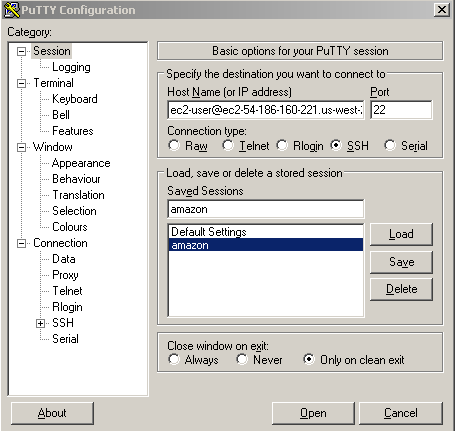
\includegraphics[scale=0.6]{putty.png}
\end{center}
\caption{PuTTY Configuration}
\label{fig:putty}
\end{figure}

In order to connect to the server, a secure key was generated by Amazon, and provided to a SSH client, PuTTY, shows in Figure~\ref{fig:putty}. This allowed access to the server, where Tomcat and MySQL servers could be installed. In order to run the application, a WAR file of the application and its dependencies was needed. A WAR, or Web application ARchive, file is a archive of the project folder structure with .class files, and .jar files for the various dependencies.  Spring Tool Suite provides functionality to export a project to a WAR file. This file was uploaded to the Amazon server using WinSCP. Once the Tomcat server was running, the browser was directed to the extracted folder created by the WAR file.

An issue that arose with the configuration of the Tomcat 7 server was the specification of a DataSource class. This class was included in the project dependencies, but was not being picked up by the server, though it had been working in the development environment. The fix was to specify this class within the \textit{context.xml} file for Tomcat, as illustrated in Figure~\ref{fig:tomcatconfig}, Line 5. \newpage

\begin{lstlisting}
<Resource name="jdbc/mtc" auth="Container" type="javax.sql.DataSource"
maxActive="100" maxIdle="30" maxWait="10000" username="root"
password="root" driverClassName="com.mysql.jdbc.Driver"
url="jdbc:mysql://localhost:3306/mtc"
factory="org.apache.commons.dbcp.BasicDataSourceFactory"
/>

\end{lstlisting}
\begin{figure}[H]
\caption{Tomcat 7 Amazon Configuration}
\label{fig:tomcatconfig}
\end{figure}

\section{External Code}
There are two aspects of external code being used within this web application. The first is the CSS file that the site is using. This was a free template obtained from \href{http://skylinestemplates.blogspot.ie/2011/11/greefies-solution-xhtml-and-css.html}{Skylines Templates}. This template was modified in order to fit in with certain aspects of the site, but the look, feel and images remain consistent with those of the template.

The other code used in this application that was not original is the Google Maps script, visible in the Contact Us page of the web application. This is provided at \href{https://developers.google.com/maps/documentation/javascript/examples/map-simple}{Google Maps Simple Map Example} and is available to use freely. 

\begin{lstlisting}
//code to include maps.jsp in contactus.jsp
<div align="center"><%@include file="maps.jsp"%></div>

//code of the maps.jsp change with modified Google javascript
<script src="http://maps.googleapis.com/maps/api/js?sensor=false">
</script>
<script>
function initialize()
{
var mapProp = {
center:new google.maps.LatLng(52.6565176,-8.5537577), //GPS Co-ords
zoom:18, // Zoom level
mapTypeId:google.maps.MapTypeId.ROADMAP
};
var map=new google.maps.Map(document.getElementById("googleMap"),mapProp);
}
google.maps.event.addDomListener(window, 'load', initialize);
</script>

\end{lstlisting}
\begin{figure}[H]
\caption{Code Showing Google Maps Integration}
\label{fig:googlemaps}
\end{figure}

The code was slightly modified, as depicted in Figure~\ref{fig:googlemaps}, to change both the GPS co-ordinates and the initial zoom level of the map. The page is included in the Contact Us tile.\newline
